\section{Logica di Distribuzione}

	\begin{figure}[htbp]
		\begin{center}
			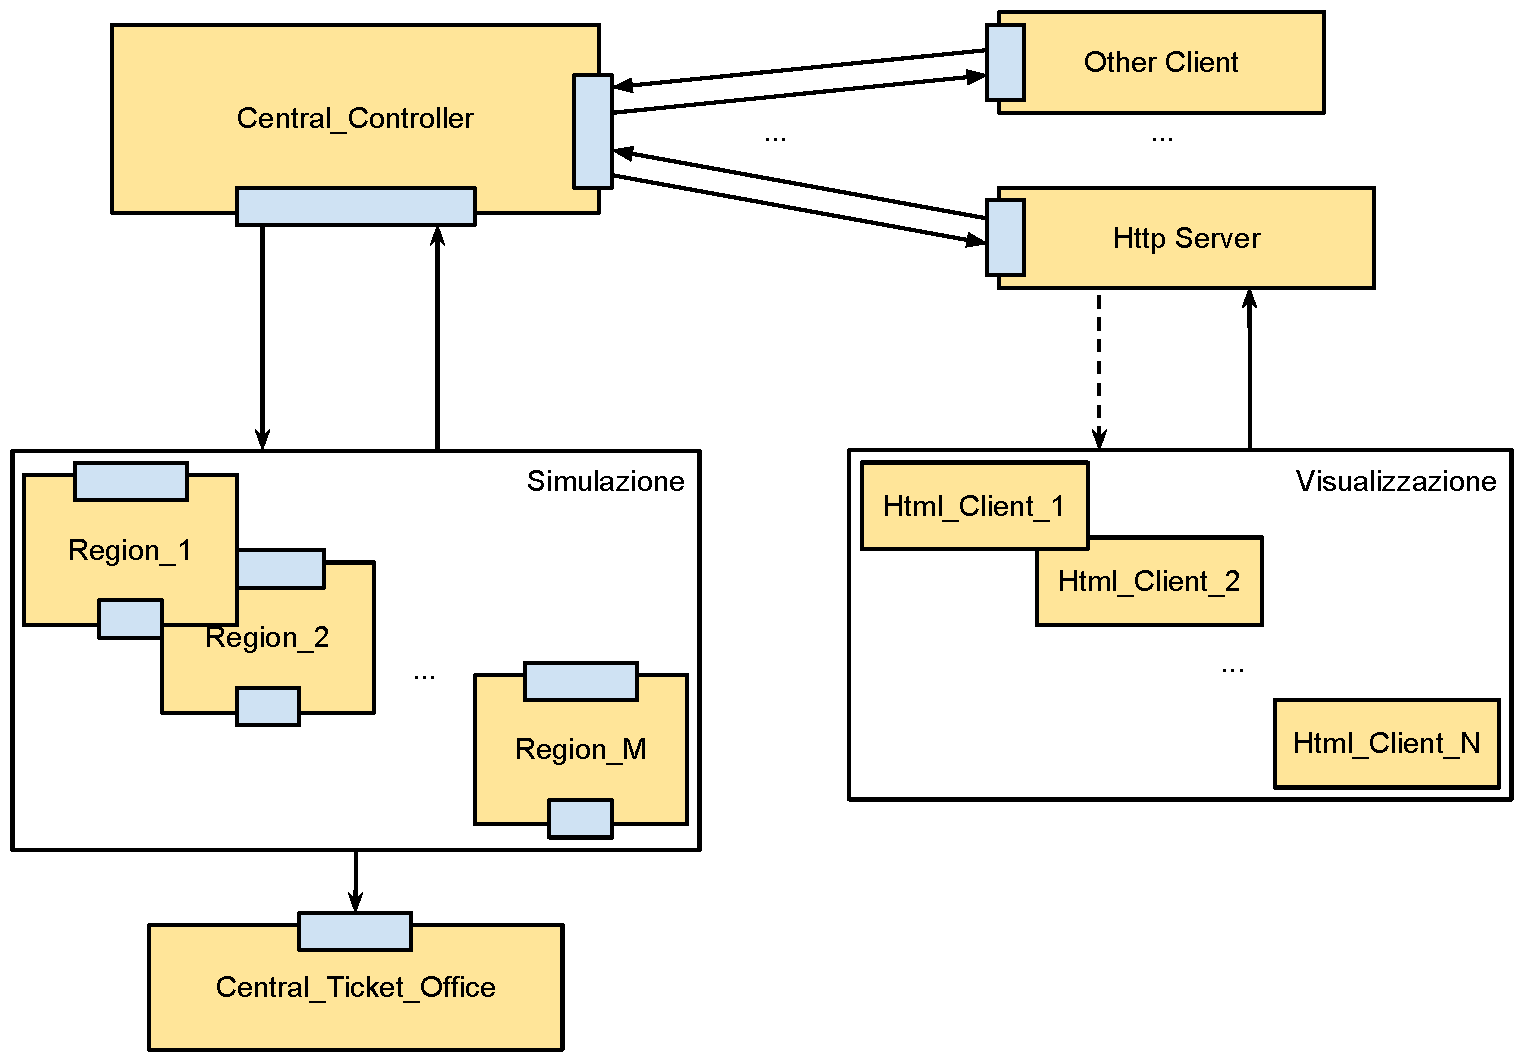
\includegraphics[width=\textwidth,keepaspectratio]{imgs/logic_distribution.pdf}
			\caption{\footnotesize{Diagramma informale che presenta una progettazione logica delle componenti distribuite.}}
			\label{fig:logic_distribution}
		\end{center}
	\end{figure}

Un diagramma infromale delle componenti distribuite che compongono il sistema è presentato in figura \ref{fig:logic_distribution}. Di seguito verranno descritte le principali.
	
	\subsection{Regioni}\label{sec:distr_regioni}
	
	La simulazione è stata suddivisa in \ii{Regioni}, le quali risiederanno su nodi di calcolo diversi. Questa scelta aggiunge i seguenti requisiti minimi alla specifica iniziale:
	\begin{itemize}
		\item I Treni, se previsto dal percorso, possono viaggiare da una Regione all'altra.
		\item I Passeggeri possono raggiungere destinazioni in Regioni diverse.
		\item Esisteranno punti di collegamento che permettono a Treni e Passeggeri di raggiungere Regioni diverse. 
		\item Deve essere garantita consistenza temporale nel passaggio da una Regione ad un'altra.
	\end{itemize}
	Da questa scelta consegue inoltre l'introduzione di un semplice \ii{Server dei Nomi} che mantiene traccia di ciascuna Regione, in modo tale da rendere agevole la risoluzione della locazione alla quale l'entità si trova. 
	
	
	\subsubsection{Stazioni di Gateway}\label{sec:gateway_stations}
	
	\begin{figure}[htbp]
		\begin{center}
			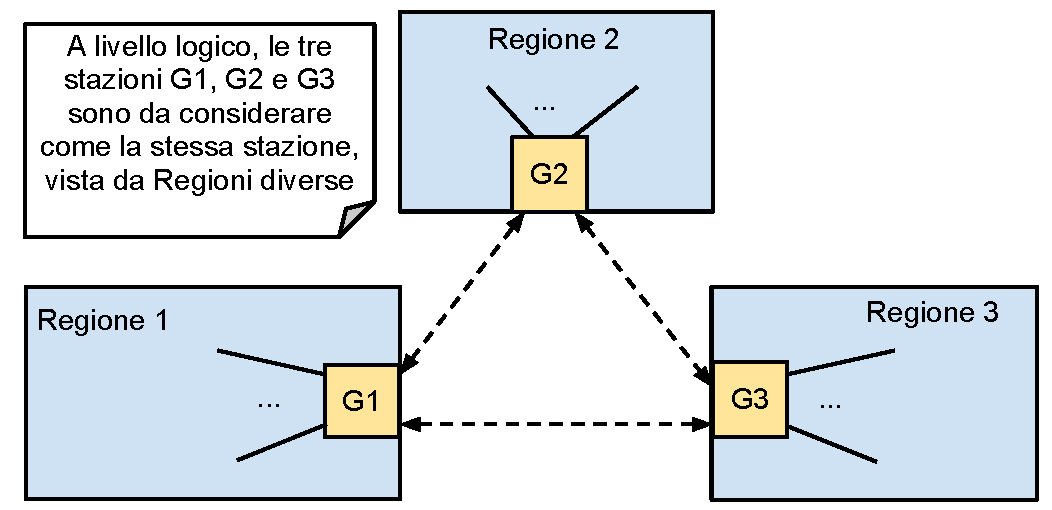
\includegraphics[width=\textwidth,keepaspectratio]{imgs/gateway_stations.pdf}
			\caption{\footnotesize{Utilizzo di stazioni di Gateway per collegare tre Regioni.}}
			\label{fig:gateway_stations}
		\end{center}
	\end{figure}

	Nella progettazione di un simulatore distribuito su più Regioni, è necessario prevedere uno o più punti di collegamento tre di esse. A tal proposito, il progetto prevede \ii{Stazioni di Gateway} (\ttt{Gateway\_Station}), che permettono di raggiungere determinate Regioni remote. Le Stazioni di Gateway che collegano $N$ Regioni in modo diretto, sono da considerare come un'unica Stazione logica, e ciascuna delle $N$ Stazioni può essere vista come una porzione della Stazione globale accessibile dalla Regione corrente. Una rappresentazione dell'idea generale è visibile in figura \ref{fig:gateway_stations}.
	
	Da tale assunzione, ricaviamo la seguente conseguenza:
	\begin{consequence}\label{cons:gateway_unique}
	Per ogni coppia $G$ e $G'$ di Stazioni di Gateway connesse (ovvero mutuamente raggiungibili in modo diretto) appartenenti a Regioni diverse rispettivamente $R_G$ ed $R_{G'}$, $\nexists$ altra Stazione di Gateway $G'' \in R_{G'}$ tale per cui $G''$ è connesso a $G$.
	\end{consequence}
	
	Per evitare sincronizzazioni tra thread distribuiti, sono posti dei vincoli nella struttura interna di questo tipo di stazoni. Ciascuna Stazione di Gateway $G$ sarà dotata di un numero $M$ di Piattaforme $\{P_1,...,P_M\}$. Le Piattaforme saranno tali da permettere un \ii{unico senso di percorrenza} delle Piattaforme, ovvero:
		
		\begin{itemize}
			\item Le prime $\{P_1,...,P_K\}$ saranno disponibili all'accesso dalla Regione in cui $G$ risiede.
			\item Le Piattaforme $\{P_K+1,..,P_M\}$ saranno invece dedicate all'accoglimento di Treni provenienti da nodi diversi.
		\end{itemize}.
	
	Questa scelta, vincola così il numero di Piattaforme per Stazione di Gateway: 
	
	\begin{consequence}
	Date N Stazioni di Gateway connesse, sia K\_i il numero di Piattaforme che permettono ad un Treno di lasciare la Regione i-esima; allora ciascuna Stazione dovra complessivamente mantenere un numero di Piattaforme pari a $\sum_{i = 1}^{N}{K_i}$.
	\end{consequence}
	
	 Tali vincoli sono sufficienti a mantenere locale ai nodi la sincronizzazione tra i thread che permettono l'esecuzione dei Treni. Una descrizione dettagliata del protocollo di accesso alle Stazioni di Gateway e di migrazione dei Treni, e presentata in sezione \ref{subsubsec:gateway_stations_func}.
	Per una descrizione dell'entità e del ruolo delle Piattaforme, si rimanda alla sezione \ref{subsec:station}

% #################################################################################################################
% ############################################### BIGLIETTERIE ####################################################
% #################################################################################################################	

	\subsection{Biglietterie}
	
	Per poter gestire meglio la definizione di un percorso e l'erogazione di un Biglietto per un Viaggiatore, ho pensato di introdurre una gerarchia su due livelli, di Biglietterie. Ci saranno dunque tre categorie di Biglietterie:
		\begin{description}
			\item {\bb{Biglietterie di Stazione}} \\
			Forniscono un'interfaccia adeguata ai Viaggiatori per poter acquistare un biglietto.
			\item {\bb{Biglietterie Regionali}}\\
			Hanno conoscenza regionale della topologia del grafo composto da Stazioni e Segmenti.
			\item {\bb{Biglietteria Cantrale}} \\ 
			Ha conoscenza di più alto livello; in particolare, essa mantiene traccia delle connessioni tra le varie regioni ( ovvero i collegamenti tra Stazioni di Gateway di regioni diverse).
		\end{description} 
	
	\subsection{Controller Centrale}
		
	Il Conterollo Centrale è una entità distribuita, alla quale tutti i nodi inviano Eventi per notificare lo stato di avanzamento globale della simulazione. Esso fornisce una interfaccia alle varie Regioni per ricevere gli Eventi di simulazione, ed un'interfaccia per permettere a client remoti di poter visualizzare gli effetti di tali Eventi. Quest'ultima possibilità è ottenuta mediante un meccanismo di tipo Publish/Subscribe, attraverso il quale client remoti possono registrarsi presso il Controller per ricevere, in modalità Push, gli Eventi.
	In questo modo è possibile per un qualsiasi client interfacciarsi al Controller e fornire, ad esempio, una rappresentazione grafica della simulazione.

	Il Controller sarà anche responsabile dell'invio di un \ii{segnale di terminazione}, che verrà recapitato a tutti i nodi che componegono la simulazione, mediante un algoritmo di Snapshot Distribuito, descritto in sezione \ref{sec:distributed_termination}.
\newpage
